\newpage
\subsection{Verification of a bolted joint}
	\paragraph{Problem} To stir the fluid contained in a cylindrical tank the system in figure \ref{ex:stirred} is adopted. It consist of a rotating arm carrying two bladed; the application point of the resulting force on the blades is indicated with dots in figure \ref{ex:stirred}; the forces are proportional to the peripheral velocity of the blades and normal to their surface. The arm is fixed to the driving shaft through a bolted joint and supported at the opposite end on a roller. Self-weight can be neglected.
	
	It is requested to
	\begin{itemize}
		\item select bolts; \item define their preload; \item do the friction verification assuming the memeber's stiffness much higher than that of the bolts.
	\end{itemize}
	
	It's known the power $P = 5kW$ applied on the system, the angular velocity $n=5rev/min$; geometrical properties: $L_1 = 400mm, L_2 = 1\,200mm, H =1\,400mm, W=150mm,B=120mm, h=20mm$. Friction coefficient $f=0.25$; safety factor against slippage $\phi= 1.25$.
	
	\begin{figure}[bht]
		\centering 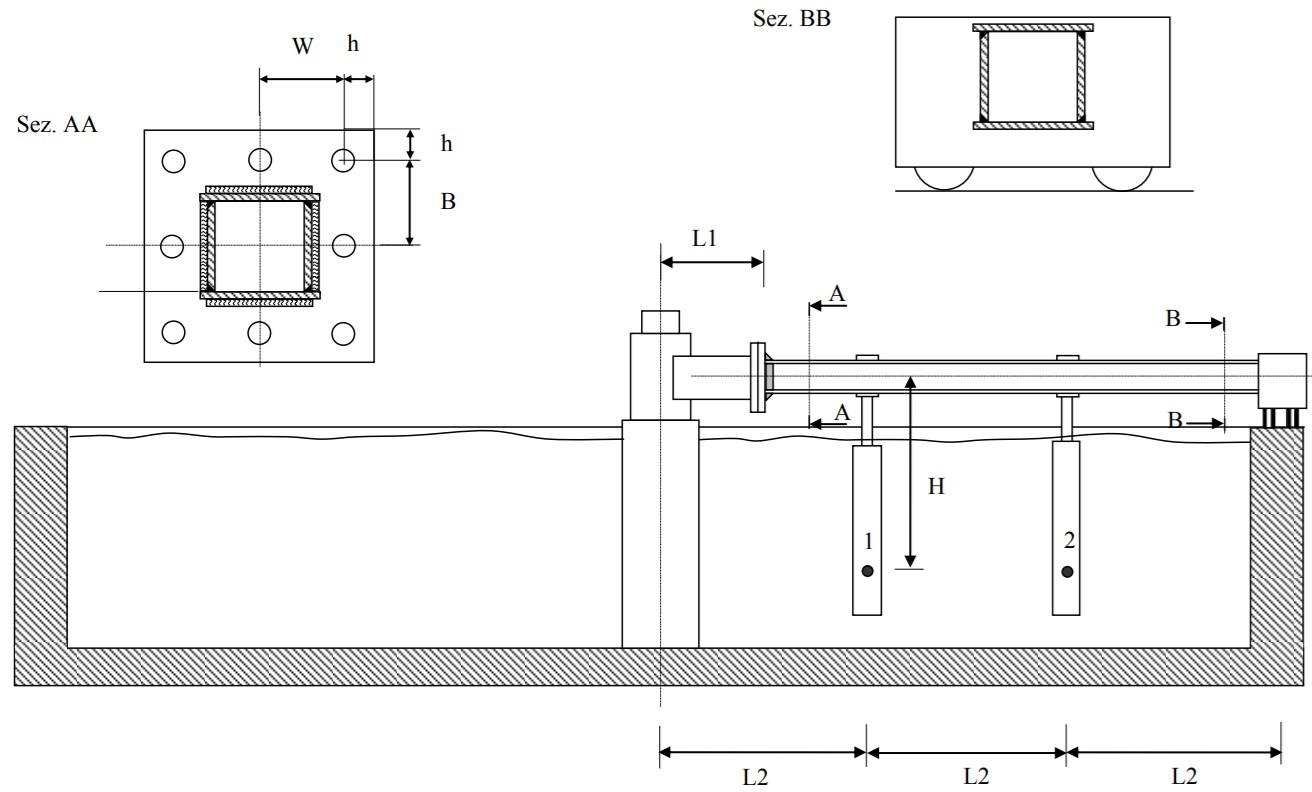
\includegraphics[width=13cm]{boltedex}
		\caption{sketch of the system used to stir the fluid.} \label{ex:stirred}
	\end{figure}
	
	\paragraph{Solution} To start the analysis we compute the torque $T$ generated by the motor; considering that $\omega = \frac {2\pi}{60}n$ such value is
	\[ T = \frac{P}{\omega} = \frac{60T}{2\pi n} =9\,549 N\cdot m  \]
	Such torque must be equated by the forces applied on the blades; in particular knowing that the forces are proportional to the velocity we have $F_1 = \alpha \omega L_2$ and $F_2 = 2\alpha \omega L_2$; computing the torque respect to the rotating axis we have
	\[ T = L_2 F_1 + 2 L_2 F_2 = 5  \alpha \omega L_2^2 \qquad \Rightarrow \quad \alpha = \frac{T}{5\omega L_2^2} = 2\,533 N\cdot s/mm  \]
	determining the forces $F_1 = 1\,591 N$ and $F_2 = 3\,183N$. From the free body diagram (figure \ref{ex:stirfbd}) we have the reactional action $R_{Ax} = F_1 +F_2 = 4\,774N$.
	
	\begin{SCfigure}[1][bht]
		\centering 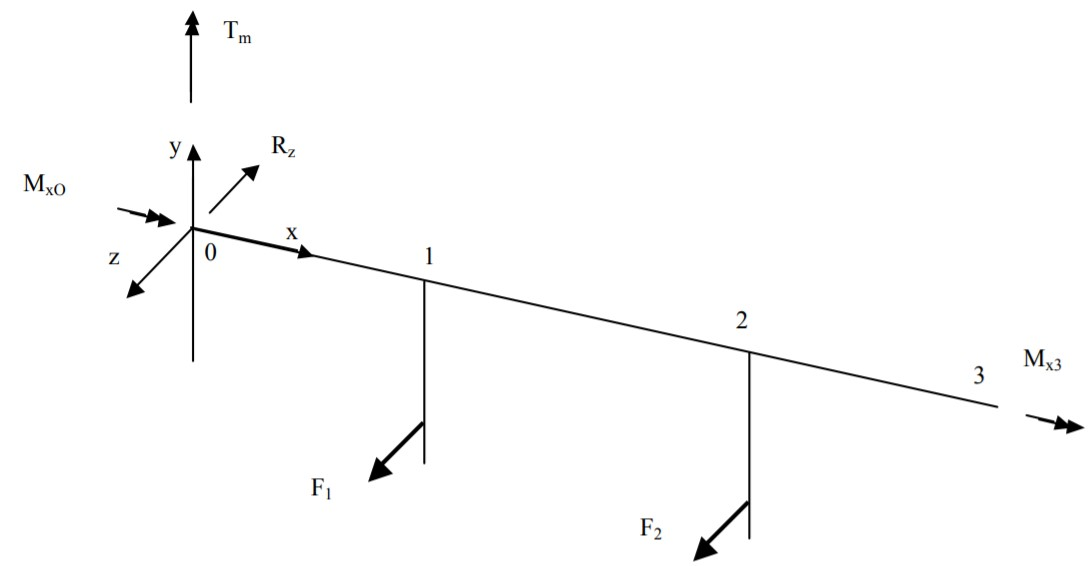
\includegraphics[width=9cm]{boltedex-reaz}
		\caption{free body diagram of the problem.} \label{ex:stirfbd}
	\end{SCfigure}
	
	\noindent
	More complex is instead the solution of the reactional moments $M_{Az},M_{Dz}$ due to having an hyperstatic problem of the form
	\[ M_{Az} + M_{Dz} = \big(F_1 + F_2\big)H \]
	A solution can be obtained by using Castigliano's theorem by firstly computing the elastic potential energy considering the hyperstatic variable $X= M_{Az}$:
	\[ U_e = \int_\Gamma \frac{M_z^2}{2GJ_t} \, dz = \frac{X^2}{2GJ_t} L_2 + \frac{(X - F_1H)^2}{2GJ_t}L_2 + \frac{(X-F_1H-F_2H)^2}{2GJ_t}L_2 \]
	Imposing 
	\[ \eta = \frac{\partial U_e}{\partial X} = \frac{L_2}{GJ_t} \big(X + X - F_1 H - F_1H-F_2H\big) = 0 \]
	we can solve for the hyperstatic variable $X$ giving
	\[ X = M_{Az} = \frac H 3 \big(2F_1 + F_2\big) = 2\,971 N\cdot m \qquad \Rightarrow \qquad M_{Dz} = H \big(F_1+F_2\big) - X = 3\,713 N \cdot m  \]
	
	With all this data retrieved is possible to compute the internal loads that the bolded connection must bear; in particular there's a shear action $V = R_{Ax} = 4\,774N$, a torque moment $M_z = X = 2\,971 N\cdot m$ and a bending evaluated as
	\[ M_y = T - R_{Ax} L_1  = 7\,639 N\cdot m \]
	\begin{SCfigure}[1.3][b]
		\centering 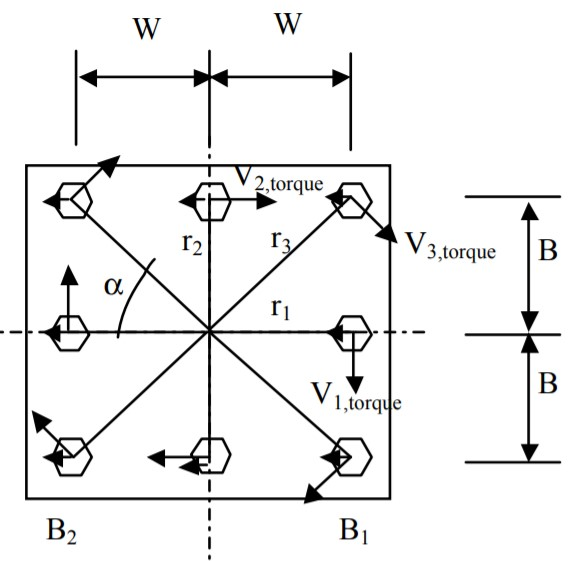
\includegraphics[width = 5cm]{boltedex-tang}
		\caption{schematic representation of the sliding actions due to shear and torque. }
		\label{ex:slidedir}
	\end{SCfigure}
	The distribution of the sliding action (considering that all bolts are equals) regarding shear can be simply calculated as $V_{i,s} = V/8 = 896.9N$; to compute instead the sliding actions due to the torque moment (whose distribution can be seen in figure \ref{ex:slidedir}) we have to consider the radii $r_1 = W = 150mm$, $r_2 = H = 120mm$ and $r_3 = \sqrt{r_1^2 + r_2^2} = 192.1mm$. Considering that
	\[ M_z = \sum_i \gamma r_i^2 \qquad \Rightarrow \quad \gamma = \frac{M_z}{2r_1^2 + 2r_2^2 + 4r_3^2} = 43\,131 N\cdot m \]
	This gives sliding forces equal to $V_{1,t} = 2\,012N$, $V_{2,t} = 1\,610 N$ and $V_{3,t} = 2\,578N$ that must be vectorially summed to the actions due to shear; in this case we see that the bolts on the bottom corners ($B_1,B_2$) are the most stressed, and in particular we have
	\[ V_{3,t,x} = V_{3,t} \cos\alpha = V_{3,t} \frac{r_2}{r_3} \hspace{2cm}  V_{3,t,x} = V_{3,t} \sin\alpha = V_{3,t} \frac{r_1}{r_3}  \]
	\[ \Rightarrow \qquad V_{tot} = \sqrt{ \big(V_{3,t,x} + V_{i,s}\big)^2 + V_{3,t,y}^2 } = 2\,987 N \]
	
	To analyse the separating action we can use the assumption of rigid members; having a positive valued $M_y$ we start off evaluating the coordinates $z_i$ of the bolt starting from the left edge. Considering that $z_1 = h = 20mm$, $z_2 = h + W = 170mm$ and $z_3 = h + 2W = 320mm$ we can find the solution for the separating loads:
	\[ M_y = \sum_i \kappa r_i^2 \qquad \Rightarrow \quad \kappa = \frac{M_y}{3z_1^2 + 2z_2^2 +3 z_3^2} = 20\,860 N/m \]
	With this theory we have that the most critical bolt is $B_1$ with a separating load of $N_3 = \kappa z_3 = 6\,676 N$.
	\begin{SCfigure}[2][t]
		\centering 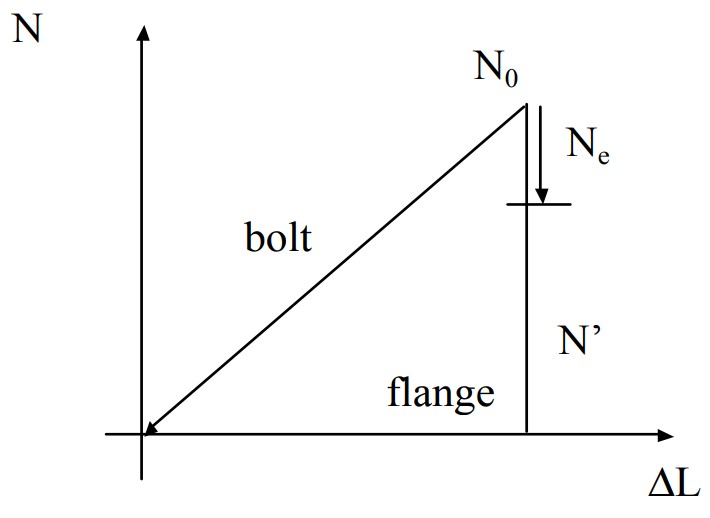
\includegraphics[width=5cm]{ex-relief}
		\caption{relieved action $N_e$ and residual preload $N'$ starting from a preload $N_0$ in the assumption of infinitely rigid member} \label{ex:reliefload }
	\end{SCfigure}
	In standard ruling the design of steel constructions, if not specified, it is allowed to consider the members as infinitely rigid compared to the bolt, so that the separating action $N_e$ (that in this case is the action that's used as load for friction) is completely absorbed by the members unloading:
	\[ N' = N_0 - N_e \]
	For friction verification this hypothesis is cautionary. The standard prescribes that the assumption of rigid members can be used only if it's verify
	\[ N_e \leq 0.8 N_0 \]
	To perform a friction verification we have to satisfy the equation
	\[ V_{tot} \leq \frac f \phi N' = \frac f \phi \big(N_0-N_e\big) \qquad \Rightarrow \quad N_0 \geq \frac \phi f V_{tot} + N_3 = 21\,611 N \]
	
	To continue the verifications (for static failure) it's necessary to consider the yield stress depending on the property class; for bolted joint working by friction, a minimum property class of 8.8 is recommended hence $\suts = 800MPa$ and $\sys = 640MPa$. Considering that the initial preload cannot exceed the value $0.8 N_{ys}$, than using a small margin of $0.05$ we get
	\[ N_0 = 0.75 N_{ys} = 0.75 \sys A_b  \]
	Having
	\[ N_0 = 0.75 \sys A_b \geq \frac \phi f V_{tot} + N_3 \]
	then the estimation of the minimum resisting cross-section of the bolts is regarded as
	\[ A_{bt} \geq \frac{\frac \phi f V_{tot} + N_3}{0.75 \sys} = 45.03mm^2 \]
	satisfying the requirement $N_e = 6\,676 \leq 17\,288 = 0.8 N_0$. By looking at table \ref{tab:bolts} a good (usual) choice is the \texttt{M10} thread with a resisting cross-sectional area $A_{bt} = 52.3mm^2$.
	 
	
	
	
	
	
	